%
% File acl2012.tex
%
% Contact: Maggie Li (cswjli@comp.polyu.edu.hk), Michael White (mwhite@ling.osu.edu)
%%
%% Based on the style files for ACL2008 by Joakim Nivre and Noah Smith
%% and that of ACL2010 by Jing-Shin Chang and Philipp Koehn


\documentclass[11pt,letterpaper]{article}
\usepackage[letterpaper]{geometry}
\usepackage{acl2012}
\usepackage{times}
\usepackage{latexsym}
\usepackage{amsmath}
\usepackage{multirow}
\usepackage{graphicx}
\usepackage{tabularx}
\usepackage[xcdraw]{xcolor}
%\usepackage{fontspec}
%\usepackage{polyglossia}
%\setmainlanguage{english}
%\setotherlanguage{arabic}
\usepackage{url}
\makeatletter
\newcommand{\@BIBLABEL}{\@emptybiblabel}
\newcommand{\@emptybiblabel}[1]{}
\makeatother
\usepackage[hidelinks]{hyperref}
\DeclareMathOperator*{\argmax}{arg\,max}

\setlength\titlebox{6.5cm}    % Expanding the titlebox
\title{Neural and Symbolic Arabic Paraphrasing with Automatic Evaluation}

\author{Fatima Al-Raisi \\
 Carnegie Mellon University \\
  School of Computer Science \\
 % Affiliation / Address line 3 \\
  {\tt fraisi@cs.cmu.edu} \\\And
 Abdelwahab Bourai\\
 Carnegie Mellon University \\
  School of Computer Science \\
  %Affiliation / Address line 3 \\
  {\tt abourai@andrew.cmu.edu} \\\And
  Weijian Lin \\
 Carnegie Mellon University\\
 School of Computer Science \\ 
 %5000 Forbes Avenue, Pittsburgh, PA 15213 \\
  {\tt wlin1@cs.cmu.edu} \\}

\date{}

\begin{document}
\maketitle
\begin{abstract}

	We present a tool for Arabic paraphrasing that yields good paraphrasing accuracy.  We present and compare several methods for paraphrasing and obtaining monolingual parallel data. We also present first results on Arabic paraphrasing using neural methods. Additionally, we propose a new evaluation metric for paraphrasing that is shown to correlate highly with human judgement.
\end{abstract}


\section{Introduction}
Paraphrasing and paraphrase detection are two important problems in natural language processing. Paraphrasing-based applications include text simplification and text generation form structured knowledge~\cite{parasimple}. Other paraphrastic models include machine translation and sentence summarization~\cite{app1,app2,app3}. Paraphrases are useful not only in generation tasks but also in analysis tasks such as information retrieval and question answering~\cite{app4,app5,app6}.\\
We present and compare two different approaches for sentence paraphrasing in Arabic: a phrase-based method and a neural method. To our knowledge, this is the first work on sentence paraphrasing for modern standard Arabic.\\ 
We also present a novel approach for obtaining parallel monolingual data and use the acquired data to train our neural sequence-to-sequence model.\\ 
As a by-product of this exercise, we contribute a large parallel monolingual corpus for Arabic containing two million sentence pairs. We also build a phrase database for Arabic containing over 88K phrase pairs of various lengths.\\ 
Another contribution of our work is devising and testing a new evaluation metric for paraphrasing. We present encouraging initial results in this paper.\\
The remainder of this paper is structured as follows: we contextualize our work within paraphrasing research in Section~\ref{related}, we present the phrase-based and neural approaches for paraphrasing sentences and building phrase dictionaries in sections~\ref{pb} and~\ref{pg}. We present details and discuss  experiments on the evaluation metric in Section~\ref{eval}. We conclude with plans for future extensions of the work.

\section{Related Work}
\label{related}
The paraphrase database project PPDB has paraphrase resources for multiple languages~\cite{bannard2005bilingual}, including Arabic. The paraphrases are obtained using parallel bilingual corpora  by applying the pivot method where one language is used as a bridge or intermediate meaning representation~\cite{bannard2005bilingual}. Paraphrases from dialectal Arabic to standard Arabic have been used in~\cite{Salloum:2011:DSA:2140533.2140535} to improve Arabic-English statistical machine translation. Turker assisted paraphrasing has been used in~\cite{turker} to improve English-Arabic MT. A comparison between various paraphrase acquisition techniques on sentential paraphrasing is given in ~\cite{Bouamor2010} but does not include experiments on Arabic sentential paraphrasing.

\section{Extracting Paraphrases from Bilingual Data}
\label{pb}
Our first approach to Arabic paraphrasing is the pivot method proposed by Bannard and Callison-Burch~\cite{bannard2005bilingual}. A key benefit is that it is language-agnostic and is based on the idea that any two source strings $e_1$ and $e_2$ that both translate to a reference string $f_1$ have similar meaning. Bannard and Callison-Burch used English as the reference string $f$, but in our study we will instead pivot into English to obtain paraphrase pairs~ \cite{bannard2005bilingual}. We obtain the final paraphrase probability by marginalizing over the English translation probabilities with $e$ and Arabic phrases $a_1$ and $a_2$. A mathematical formulation of the approach can be found in Equation~\ref{eq1}.

\begin{equation}
p(a_2 | a_1) = \sum_{e} p(a_2 | e) p(e | a_1)
\label{eq1}
\end{equation}

In order to extract paraphrases, we first obtained a parallel bilingual corpus through English and Arabic versions of the EUROPARL dataset \cite{Koehn_europarl}. We pruned the corpus to only contain sentences with less than 80 words and tokenized using the StanfordNLP Arabic Tokenizer~\cite{manning}. This gave us a final corpus size of 241,902 sentences.\\ 
Additionally, to calculate conditional probabilities for our paraphrase equation, we need alignments. Thus we ran GIZA++ to obtain these alignments \cite{och03:asc}. Once we have a database of paraphrase mappings, we can then substitute phrases with their corresponding paraphrases by selecting the phrase with the highest probability. This substitution approach was used by Bannard and Callison-Burch in their study as well \cite{bannard2005bilingual} The way we extract the paraphrase is summarized in Equation~\ref{eq2}. 
\begin{equation}
\hat{a_2} = \text{argmax}_{a_2 \neq a_1} p(a_2 | a_1)
\label{eq2}
\end{equation}
An example of this process can be seen in Figure~\ref{fig:pivot}
\begin{figure}
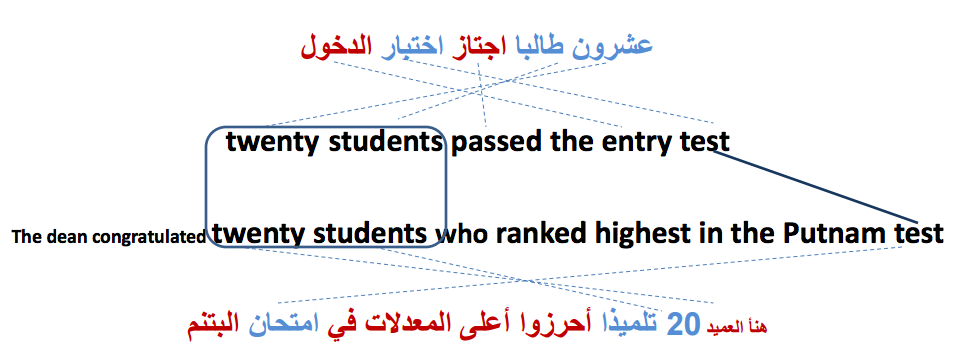
\includegraphics[scale=0.25]{arabic_pivot}
\caption{An example paraphrased sentence produced using the pivot method. }
\label{fig:pivot}
\end{figure}
\subsection{Improving Coverage of Phrase Database}
In our initial experiments, we noticed that generated phrase pairs did not necessarily match in some grammatical features such as definiteness and number. We post-processed the phrase dictionary to add entries with other variants of the phenomenon for completion. For example, for a word pair that appears in the phrase table where one word is definite and the other is not, we add two entries where both are definite and both are indefinite. We did not adjust the scores to reflect this but ordered the entries according to observed frequency of the word/phrase. For definiteness, we limited the addition to the clear definite marker ``al-'' in Arabic. We applied the same for simple cases of number matching where the morphology is concatenative or easily processed. We note that this modifications did not include all  possible mismatches since they were based on simple heuristics. However, this may have contributed to better grammaticality as  discussed in Section~\ref{earlyresults}.\\
We also noticed cases like the following in the generated phrase table:
\begin{center}
x $\vert\vert\vert$ y $\vert\vert\vert$ score\\
x $\vert\vert\vert$ z $\vert\vert\vert$ score\\
\end{center}
We included, for improved coverage, the following entry:
\begin{center}
y $\vert\vert\vert$ z $\vert\vert\vert$ score\\
\end{center}
Again, this was limited in scope since we relied on simple string match to identify such entries. 
\subsection{Phrase-substitution}
We randomly sampled 100 sentences from the datasets we have~\cite{data1,data3} and performed phrase substitution. Figure~\ref{sample1} 
shows a sample of paraphrased sentences acquired using phrase substitution. We note that in the last example the output sentence differs from the original in only one word (last word) but the meaning is entirely altered. We discuss results and experiments on the quality of paraphrased sentences in Section~\ref{earlyresults}.
\newpage
\begin{figure*}[h!]
\center
%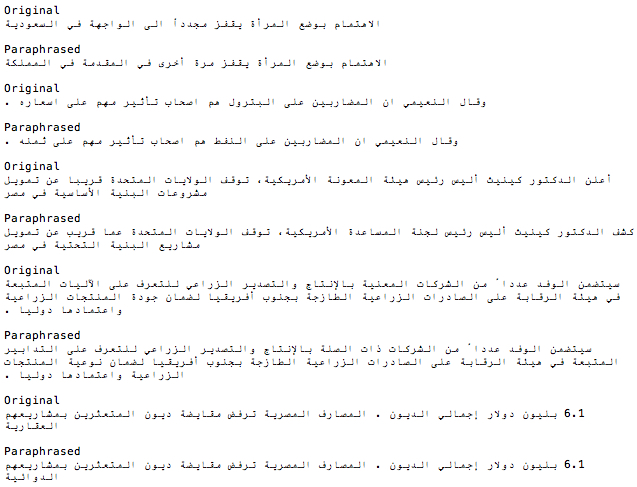
\includegraphics[clip=true,trim={0 7cm  0 0},width=\textwidth]{sampleoutput1a.jpg}
\frame{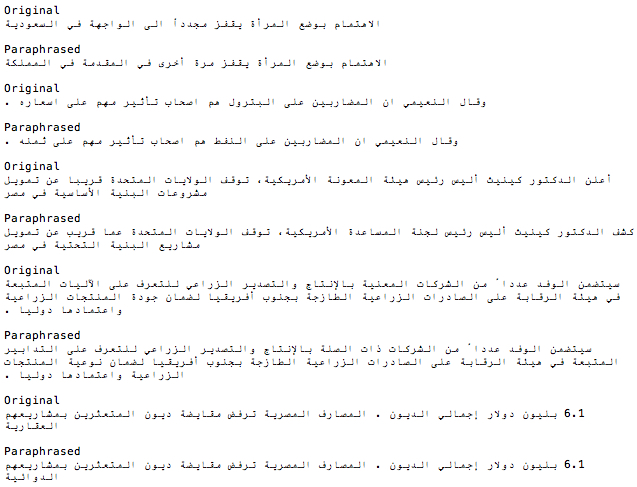
\includegraphics[width=\textwidth]{sampleoutput1a.jpg}}
%\frame{
\caption{Sample output produced using phrase substitution}
\label{sample1}
\end{figure*}
\section{Monolingual Parallel Data for Seq-to-Seq Paraphrasing}
\label{pg}
We need parallel monolingual data to train our sequence-to-sequence paraphrasing model. To address the lack of parallel monolingual data for Arabic, we propose a novel method for generating Arabic parallel language sentences using two other language pairs as resource. The idea is to use paired sentences data from two other languages, translate them into Arabic correspondingly, then use them as the  training data for sequence-to-sequence machine translation model to train a translator  to generate Arabic to Arabic paraphrases.\\  
The first advantage of this approach is its scalability. After preparing enough training data for the paraphrase model, the generation step for Arabic paraphrases is easily scalable. The second advantage is that the seq-to-seq paraphraser model may contain valuable insight for  building Arabic paraphrases database at  words and phrases level, since state of the art neural machine translation techniques are capable of capturing word and phrase level similarity by projecting word embeddings into vector space.\\
We used europarl-v7 fr-en~\cite{Koehn_europarl} data which contains two million sentence pairs, and then used Google translate API to generate French-Arabic and English-Arabic sentence pairs correspondingly. Then we paired the output to construct parallel monolingual data and used it as training data for a Bi-LSTM with embedding size and hidden size set to be 512 and attention size set to be 128. The whole process is demonstrated in Figure~\ref{fig:mono}. Training the Bi-LSTM took about 7 days on this dataset and we obtained a corpus of monolingual Arabic containing two million parallel sentences.\\ 
\begin{figure}
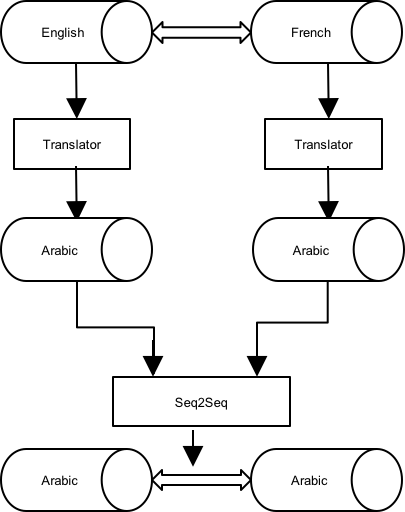
\includegraphics[scale=1.0]{monolingual}
\caption{Overview of the process completed to obtain two parallel Arabic corpora generated from different source languages}
\label{fig:mono}
\end{figure}
\section{Results}
\label{earlyresults}
We report results on the bilingual pivot and sequenc- to-sequence approaches detailed above. 
\subsection{Phrase-based Method}
Using the pivot method, we obtained over 88K phrase pairs. We report a few results. First, Figure~\ref{fig:para_length} shows the length distribution for phrases in the database.\\ 
\begin{figure}[h!]
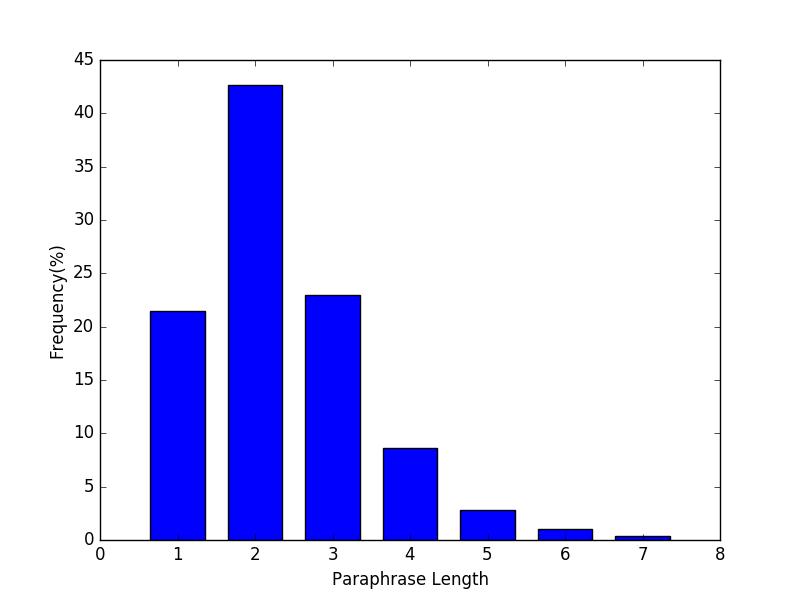
\includegraphics[scale=0.4]{phrase_len}
\caption{Distribution of phrase lengths in our paraphrases obtained through pivoting}
\label{fig:para_length}
\end{figure}

\noindent We obtained human evaluations from two native speakers on the grammaticality and  meaning preservation aspects of the paraphrased sentences. For each criterion, we asked the annotator to judge the quality of the output on a scale from 1 to 5. We chose this scale to capture variation in the level of grammaticality (since there are minor and more serious grammatical mistakes) and in the extent to which the paraphrased sentence preserved the meaning of the original sentence. The agreement between annotators calculated in terms of IntraClass Correlation, preferred for ordinal data, is summarized in Table~\ref{ann1}. It was not expected to find higher agreement on meaning preservation since it is more subjective than grammaticality. It is possible that phrases substituted were of similar meaning yet possibly resulted in unusual sentence structure which  made the meaning preservation judgement straightforward while grammaticality harder to judge. 
\begin{table}
\begin{tabular}{|c|c|c|}
\cline{2-3}
%\multicolumn{1}{c|}{}
\multicolumn{1}{c|}{} & ICC(single) & ICC(average) \\
\hline
Grammaticality & 0.375 & 0.545\\
\hline
Meaning  & 0.707 & 0.547\\
\hline
\end{tabular}
\caption{Inter-annotator agreement}
\label{ann1}
\end{table}
We analyzed changes made to reference sentences that received the highest score in meaning preservation after paraphrase substitution (score = 5) . A change is a word replacement or deletion. Table~\ref{parasummary} summarizes these changes. When $n$ consecutive words are replaced by $n$ or more words, we consider those to be $n$ changes rather than 1 phrasal change. 
\begin{table}
\begin{center}
\begin{tabular}{|l||c|c|c|c|c|}
\hline
 No. of changes  & 5 & 4 & 3 & 2 & 1 \\
\hline
 Frequency (Sent.) & 3 & 4 & 5 & 16 & 26 \\
\hline
\end{tabular}
\caption{Number of changes in paraphrased sentences with high meaning preservation score\label{parasummary}}
\end{center}
\end{table}
Table~\ref{evaltable} summarizes the evaluation of paraphrased sentences obtained using phrase substitution.
\begin{table}
\begin{tabular}{|c|c|c|c|}
\hline
%\multicolumn{1}{c|}{}
scale & {\small{Grammaticality}} \% &  {\small{Meaning}}  \% & Both \% \\ 
\hline
5 & 62 &	62	& 50 \\
\hline
4 & 21 &	16	& 7 \\
\hline
3 & 10 	 & 9 	& 3 \\
\hline
2 & 7 & 12 &	4 \\
\hline
1 & 0	&  1  &	0 \\
\hline
\end{tabular}
\caption{Evaluation of paraphrased sentences (averaged and rounded from two annotator ratings)}
\label{evaltable}
\end{table}
%\end{center}

As for the neural model,  the produced corpus of sentence pairs was large (2M). By the time the output was produced, we had exhausted our human evaluation resources, so we qualitatively evaluated it on a small subset consisting of the first 10 sentence pairs. Based on this small sample, the monolingual parallel sentences obtained were grammatical or near grammatical with minor mistakes and highly similar in meaning. Also, they were sufficiently different in surface form which encouraged their use as input to a seq-to-seq paraphrasing model. Initially, we were concerned of the possibility that the en$\rightarrow$ar and fr$\rightarrow$ar translation tools we used were trained on the same Arabic dataset with similar model architecture and parameters, in which case the output would not be diverse enough to be useful as input to the paraphrasing system. We were also concerned of the possibility that the French source was translated to English and then to Arabic. However, judging by the clear diversity in the output of these models, we were further encouraged to use the resultant  parallel monolingual corpus to train the neural paraphrasing model. We plan to quantitatively compare the surface diversity in the output of the fr-ar and en-ar MT models by computing word overlap and hamming distance between corresponding sentences. Due to time constraints we leave this for future work.

The paraphrased output from the neural system was far from grammatical and meaning was incomplete due to early sentence truncation, especially for long sentences. Better output was observed for shorter sentences. However, we make the following observations about the output:
\begin{itemize}
\item The model learns what phrases to use at the beginning of the sentence. It uses things like ``Moreoever'' and ``As you know,'' (translated from Arabic), exactly at the beginning of the sentence.
\item The model seem to lean and include central parts of the sentence in the output such as the subject or the location of the event.
\item The model learns correspondences between  the main parts of the sentence; e.g., the byline vs. remainder of the sentence and quoted text vs. part before the quotation.
\item The model often fails in producing output with the correct word order. 
\item  As observed with neural language models, it tends to repeat words. 
\end{itemize}
Figure~\ref{sample2} shows a sample output from the neural model.
\begin{figure*}
\center
%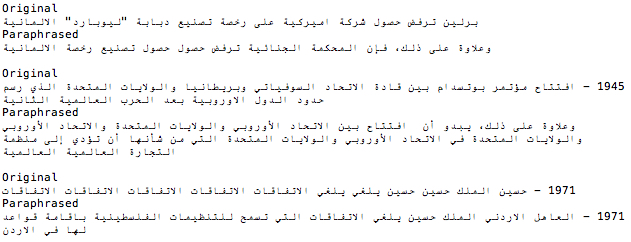
\includegraphics[clip=true,trim={0 7cm  0 0},width=0.9\textwidth]{sampleoutput.jpg}
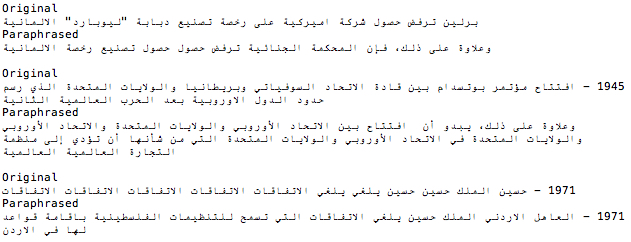
\includegraphics[width=\textwidth]{sampleoutput.jpg}
\caption{Sample output from neural parpahrasing model}
\label{sample2}
\end{figure*}

\section{An Automatic Evaluation Metric}
\label{eval}
Since human evaluation is time-consuming, subjective and not always available, we propose an automatic evaluation metric for paraphrasing. We propose criteria for judging paraphrase quality and operationalize those criteria using well-defined functions. A good paraphrase has the following two properties:
\begin{enumerate}
\item maintains the meaning of the original text, yet
\item expresses the same meaning using different surface realizations.
\end{enumerate}
To evaluate the semantic similarity and surface variation in a paraphrase we employ well-defined metrics discussed next.

\subsection{Semantic Similarity}	
Several methods exist for capturing the semantic similarity of text~\cite{sim1,sim2,sim3}. One simple approach uses the distributional properties of words in the sentence and embeds a sentence 
$x = \langle x_1, x_2, \ldots, x_n  \rangle$ by averaging the embedding vectors of its words. We choose this method for its simplicity and efficiency. The sentence vector is thus given by:
%$ w_x = \frac{1}{|x|} \sum \emph{embedding}_\theta (x_i)$\\

\begin{equation}
w_x = \frac{1}{|x|} \sum_{1}^{n} w_{x_i}
\end{equation}

where $n$ is the number of words in the sentence. 
 Although this method is simple and does not consider word-order or syntactic structure, it performs surprisingly well when compared to more advanced neural- based methods designed to capture sentential semantics~\cite{sim4}. It also correlates highly with human judgement~\cite{sim4}. Also, being agnostic to word order is actually a desired property in the paraphrase case since valid paraphrases may only differ in the order of the words or the construction used. For example, in Arabic the SVO word order can almost always be changed to VSO without changing the meaning of the sentence\footnote{except for emphasis} and without introducing any other particle. Another example is English active voice and the corresponding passive voice sentence ( + \emph{by} Subj) of the original sentence. \\
 To compute the semantic similarity between two sentences, the original sentence and the paraphrase, the cosine similarity between the two sentence vectors is computed. In our experiments, we use word embeddings with 300 dimensions trained on Arabic text from~\cite{bojanowski2016enriching}.
 
\subsection{Surface Variation}
To capture surface variation we first map each sentence into a common vocabulary space and compute the hamming distance between the sentence vectors in that space. This also limits sentence length bias where short sentences will naturally have less surface overlap. In our experiments, we map sentences into a vocabulary space of 610977 words~\cite{bojanowski2016enriching}. We present experiments and results in section~\ref{evalresult}.

\subsection{Combining Criteria for Meaning and Form}
Minimal change in surface form can result in maximal preservation of original meaning. However it will score low on surface variation. Similarly, if surface form is significantly changed, we may risk altering the meaning of the original sentence. Since semantic similarity and surface variation are two competing criteria, we combine them using (balanced) harmonic mean. The final score of the paraphrase is given by:

\begin{equation}
\emph{s} = 2\:\frac{\emph{SemanticSimilarity}\cdot\emph{LexicalDistance}}  {\emph{SemanticSimilarity}+\emph{LexicalDistance}}
\end{equation}

\subsection{Results}
\label{evalresult}
We evaluate a set of 198 Arabic sentence pairs sampled from newswire data~\cite{data3} as follows. These include  headlines on similar topics and for each headline one or two sentences detailing the event in the headline or reiterating it. Pairs including the headline and the following sentence were reasonable paraphrase pairs whereas the other pairs varied in paraphrasing potential from moderate (some overlap in meaning) to poor (unrelated, contradicting or little overlap).  We created 576 sentence pairs from the dataset but obtained annotations for only 198 of them. This evaluation of the metric was conducted before obtaining paraphrasing results from our phrase-based and neural models. Therefore, we created sentence and paraphrase pairs following this approach. Since sentences were obtained from newswire data, we assumed they are grammatical and did not obtain grammatical judgement from annotators. On paraphrastic quality, human evaluations were obtained from three annotators who are native speakers of Arabic. Each annotator was asked to judge the quality of the paraphrase, on whether it preserved meaning and was expressed differently, on a ordinal scale from 1 to 5 where 1 indicates poor quality. We used R to measure  inter-annotator (absolute) agreement using IntraClass Correlation (ICC) and agreement was measured at 0.714 ICC which is considered ``very good.'' The biserial correlation between the binarized human evaluations and the evaluation metric scores was 0.813. 
\subsection{Analysis}
Observing high correlation between human evaluation and the proposed evaluation metric, we examined the dataset to see if results were biased by sampling or data peculiarities. For sentence pairs including the headline and the following sentence, both human and evaluation metric scores were high. For most of the other sentence pairs, the paraphrase was judged as weak or poor. In both of these cases, the judgement was ``easy'' and straightforward and this perhaps lead to the surprisingly good results. Perhaps sentence pairs with finer and more subtle semantic phenomena such as polysemy and synonymy would have been harder to score accurately by the metric.  We need to conduct more experiments to verify this.\\ 
We also explored the effect of the embedding dimension on the correlation between human evaluation and the metric we proposed. We experimented with lower dimensions: 50, 100, 150, 200, 250 and obtained slightly lower values of biserial correlation as we decreased the embedding dimension. With 50 dimensions, the absolute difference between the previous biserial correlation value and the new one was 0.03. It is worth mentioning that when only using overlap as a measure of semantic similarity, the correlation between human judgement and the evaluation metric is 0.47. We clearly gain by using word embeddings but even something as simple as word overlap can capture semantic distance to some extent and explain a good amount of variation in human judgement.\\ 
\noindent We initially planned to experiment with the size of the vocabulary space in which the lexical distance between the sentence and a paraphrase is computed but due to time constraints we leave that as future work. We initially set out to compute the surface distance between two sentences using a measure that only depends on the two sentences as input; such as token/character overlap or minimum edit distance. However, we decided to compute the hamming distance in a canonical space since the first approach can have a length bias.\\ 

\noindent We also prefer using a common canonical space for doing the various computations as these spaces comprise a reference against which candidates are evaluated. When using the metric to evaluate outputs from different systems, the reference can be decided at test time to avoid ``gaming'' the metric. It is desirable to have a metric that does not require a reference sentence when evaluating a candidate paraphrase since 1. results and rankings can be sensitive to the choice of the reference sentence which is often subjective and 2. the notion of a ``reference paraphrase'' is problematic here since paraphrasing is essentially based on divergence from a given surface form while preserving the  underlying meaning and hence is loosely constrained. However, we do recognize the problem with not having a reference for an evaluation metric: it can make it susceptible to ``gaming'' by players competing to optimize the metric score. Therefore, we propose to decide the vocabulary space in which surface distance function is computed and the semantics space in which semantic similarity is computed at test time.\\ 

\noindent Also, since this metric combines competing objectives, the parameter controlling the relative strength of each component can also be decided at test time to improve the metric robustness. While it has been shown that it is possible to find a Pareto optimal hypothesis that aims to jointly optimize several different objectives~\cite{Duh:2012:LTM:2390524.2390526}, we argue that those objectives are not exactly \emph{competing} or orthogonal. They may be weakly correlated but they are still positively correlated since they compare surface distance against the same reference (as in BLUE and TER), which is not the case in our proposed metric setting.  
 
\section{Conclusion}

We presented and compared two different approaches for sentence paraphrasing in Arabic. The phrase-based approach yielded very good results when used to create paraphrase sentences. The neural method output is still far from practical applicability but the model has learned interesting linguistic constructs like phrases used for sentence opening. We also presented a novel approach for obtaining parallel monolingual data and contributed a dataset of two million parallel sentence pairs in Arabic using this approach. We applied the pivoting method to construct a large coverage paraphrase database for Arabic that includes over 88K phrase pairs. When used to create new sentences, the paraphrase dictionary gave very good results on grammaticality and meaning preservation. We proposed a new automatic evaluation metric for paraphrasing that does not require the use of a reference sentence while evaluating candidate hypotheses. We showed encouraging preliminary results in terms of correlation with human judgement. 

\section{Future Work}
 We plan to explore other options for obtaining monolingual parallel data. One possible approach is to retrieve headlines of news articles from different agencies covering the same event. We expect headlines describing the same event to have some degree of semantic similarity yet different surface realizations.\\
The sequence-to-sequence model required a relatively long time to run which limited the testing of other architectures and model parameters. We plan to conduct more experiments on different architectures and compare results. More specifically, whether we get better results with a uni-directional model since sequences from the same language will tend to have similar word order. We also intend to incorporate the concept of ``coverage''~\cite{DBLP:journals/corr/MiSWI16} to address issues with fluency of the neural model output.\\ 
We obtained encouraging results from the evaluation metric experiments but we need to verify its usefulness in settings with subtle semantic phenomena such as polysemy and synonymy. We also plan to use it at word subunits such as morphemes and even character level especially for surface distance comparison in morphology rich languages like Arabic. 

\bibliography{projectreport}
\bibliographystyle{acl2012}

\end{document}


